% #############################################################################
% This is Chapter 2
% !TEX root = ../main.tex
% #############################################################################
% Change the Name of the Chapter i the following line
\fancychapter{Conceptual Modelling}
% The following line allows to ref this chapter
\label{chap:cmodl}

This chapter presents the conceptual foundations that support the methodology proposed in this dissertation. It first relates conceptual modelling to \ac{EA}, before introducing architecture descriptions, viewpoints, and views through the concepts established by ISO/IEC/IEEE 42010. The chapter then presents ArchiMate as the modelling language used to express the resulting architectural representations and discusses the opportunities and limitations of using generative language models in modelling work. Together, these foundations establish the terminology and modelling principles used throughout the remainder of the dissertation.

% #############################################################################
\section{Conceptual Modelling and Enterprise Architecture}

Conceptual modelling is about describing the semantics of software applications at a high level of abstraction. Specifically, conceptual modellers:
\begin{itemize}
    \item Describe structure models in terms of entities, relationships, and constraints;
    \item Describe behaviour or functional models in terms of states, transitions among states, and actions performed in states and transitions;
    \item Describe interactions and user interfaces in terms of messages sent and received and information exchanged.
\end{itemize}

Although these activities are often associated with individual software applications, they are also applicable to the wider enterprise domain. Enterprise conceptual models support the understanding and communication of organisational situations by representing relevant business, organisational, information, and technical concepts at an appropriate level of abstraction. Anaby-Tavor et al. report that, in their empirical study of practice at IBM, business analysts, business architects, and solution consultants used modelling-related practices and work products to understand business contexts. Such work products could subsequently inform formal software-requirement definitions or recommendations for business activities \cite{AnabyTavorEtAl2010}.

At this broader scale, conceptual modelling and \ac{EA} are complementary. Conceptual modelling provides the means to identify and express the relevant concepts, relationships, and constraints of an enterprise. \ac{EA} provides the enterprise-wide purpose for these representations: it concerns the integrated relationships among organisational structures, business processes, information systems, and technical infrastructure. Rather than treating organisational structure, business processes, information systems, and infrastructure as independent domains, \ac{EA} provides an integrated perspective through which their relationships can be considered together. \cite{LankhorstEtAl2004}.

Consequently, an enterprise model should not attempt to reproduce every detail of an organisation. Its value lies in selecting the concepts and relationships that are relevant to a given analytical or communicative purpose, while preserving sufficient context for those selections to be interpreted. This principle is particularly important where a change, obligation, or risk crosses organisational and technical boundaries: its significance may depend on the relationship between responsibilities, processes, information, applications, and infrastructure rather than on any one element in isolation.

ISO/IEC/IEEE 42010 recognises enterprises as entities whose architectures may be expressed through structured architecture descriptions \cite{ISO42010:2022}. It therefore provides an appropriate conceptual foundation for using enterprise models to address architectural concerns without confusing a representation with the enterprise itself. In this dissertation, ArchiMate supplies the \ac{EA} modelling language used to express selected concepts and relationships in a consistent notation \cite{opengroup}. The following sections introduce the \ac{AD} concepts and ArchiMate foundations that guide this use.

\section{Architectural Descriptions, Viewpoints and Views}

In their typical usage, conceptual-model diagrams are high-level abstractions that enable clients and analysts to understand one another, enable analysts to communicate successfully with application programmers, and in some cases automatically generate (parts of) the software application\footnote{\label{fn:conceptual_modelling_conference}Taken from ConceptualModeling.org, available at \url{https://conceptualmodeling.org/ConceptualModeling.html}}.
These diagrams are implementation-independent and represent a domain's key concepts and their relationships. By abstracting away technical details, conceptual models capture the universe of discourse for a system or organization.

Conceptual modelling ensures clarity in every system design, being essential for creating clear \ac{AD}s, which formally represent system architectures\cite{Pbol}. As written in ISO 42010, an \ac{AD} is an "work product used to express an architecture", and not the architecture itself. An \ac{AD} may "take the form of a document, hypertext or a wiki, a collection of models, a repository, or some other medium"\footnote{\label{fn:iso42010}Taken from iso-architecture.org, available at \url{http://www.iso-architecture.org/ieee-1471/index.html}} and addresses stakeholder concerns through views and viewpoints\cite{Pbol}. Additionally, an \ac{AD} is made up of elements, which can be ``stakeholders, concerns, stakeholder perspectives, aspects, other \ac{AD}s (correspondences), architecture views, view components, architecture viewpoints, and model kinds''\cite{ISO42010:2022}.

These concepts are formalised in ISO 42010. The viewpoint is a set of rules used to create a view: "A set of conventions for constructing, interpreting, using and analysing one type of Architecture View. A viewpoint includes Model Kinds, viewpoint languages and notations, modelling methods and analytic techniques to frame a specific set of Concerns." These viewpoints may express operational, technical, logical or other types of concerns\footref{fn:iso42010}. According to \ac{TOGAF}, a viewpoint can also be seen as a schema for a kind of architecture view. It establishes the conventions for constructing an using a view to address a specific concern (or set of concerns) about a system-of-interest \cite{TOGAF_Intro}. The ArchiMate 3.2 Specification also provides a definition of viewpoints. They ``define abstractions on the set of models representing the \ac{EA}, each aimed at a particular type of stakeholder and addressing a particular set of concerns''. Viewpoints can also be used to view certain aspects in isolation, or to relate two or more aspects \cite{opengroup}.
For example, a governance viewpoint can concentrate on legal accountability and decision rights while an operational viewpoint can show processes, actors, information, and service dependencies. These are suitable choices for this work. A single viewpoint can govern one or more views, allowing the same modelling conventions to be reused at different levels of detail or for different stakeholder audiences \cite{ISO42010:2022}.

A view is an ``information part comprising portion of an architecture description''\cite{ISO42010:2022} that "expresses the Architecture of the \ac{EoI} from the perspective of one or more Stakeholders to address specific Concerns, using the conventions established by its viewpoint"\footref{fn:iso42010}. The \ac{EoI} refers to the subject of the \ac{AD}, which can range from software and systems to entire enterprises.

Deriving from these definitions, it can then be said that a viewpoint is a set of rules used to create, interpret,  analyse and use one type that addresses a specific set of concerns (representing different stakeholder) about an entity of interest. These concerns may take different forms, such as operational, technical or logical.

An \ac{ADL} is a language that enables enterprise architects to create comprehensive representations of it's\ac{AD}s. An example of this is ArchiMate, a ``comprehensive enterprise data modelling language that allows architects to create clear and integrated models of enterprise architecture''\footnote{\label{fn:linix}Taken from leanix.net, available at \url{https://www.leanix.net/en/wiki/ea/enterprise-architecture-frameworks}}. The ArchiMate specification emphasizes modelling with concepts, offering a comprehensive way to represent abstract structures and their relationships\cite{Pbol}. As an \ac{ADL}, ArchiMate "provides a set of entities and relationships with their corresponding iconography for the representation of Architecture Descriptions"\cite{opengroup}.

\section{ISO/IEC/IEEE 42010}

ISO/IEC/IEEE 42010:2022 provides an international basis for the structured expression of architectures. Its purpose is not to prescribe how an organisation must design a system, select a technology, or interpret a legal obligation. Instead, it specifies requirements for the structure and expression of \ac{AD}s for a broad range of entities, including software, systems, enterprises, systems of systems, products, services, technologies, and business domains \cite{ISO42010:2022}. 
ISO/IEC/IEEE 42010 offers a way to organise an architecture description of those relationships without confusing the description with the legal acts or with the architecture itself.

The distinction between an architecture and its description is fundamental. An architecture concerns the essential characteristics of an entity in its environment, whereas an \ac{AD} is the work product used to express that architecture \cite{ISO42010:2022}. In the context of legal compliance, an \ac{AD} is therefore an analytical and communicative artefact. It can show how a regulated organisation, a national implementation environment, or a cross-border service ecosystem is arranged in relation to legal obligations. It does not replace the binding text of the law, determine the final legal meaning of a provision, or prove that an organisation is compliant. Its contribution is to make the assumptions, responsibilities, dependencies, and evidence relevant to compliance visible to the people who need to inspect and discuss them.

For this purpose, the entity of interest must be defined with care. It may be an organisation subject to \ac{DORA} or another bounded implementation context. Once the entity is identified, the architecture description can identify its stakeholders and their concerns. Stakeholders may include competent authorities, regulators, enterprise architects, security managers, service providers, relying parties, system operators, auditors, and citizens. Their concerns are not identical: an authority may need assurance that responsibilities and reporting paths are clear, while a service provider may need to understand data exchanges, controls, and dependencies. ISO/IEC/IEEE 42010 treats concerns as matters of relevance or importance to stakeholders and explicitly accommodates legal and regulatory considerations among the matters that can affect an architecture \cite{ISO42010:2022}. This makes stakeholder and concern identification a substantive modelling activity rather than a preliminary administrative step.
The relationships among these central ISO/IEC/IEEE 42010 concepts are summarised in Figure \ref{fig:iso42010-concepts}.

\begin{figure}
  \centering
  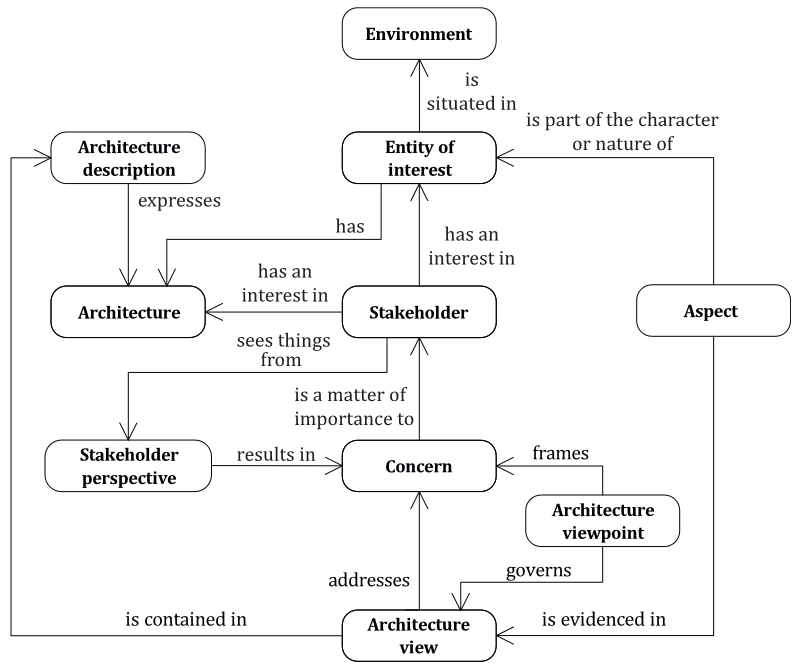
\includegraphics[width=01\textwidth]{Images/ISO_Diag.png}
  \caption{Relationships among the central ISO/IEC/IEEE 42010 architecture-description concepts \cite{ISO42010:2022}.}

  \label{fig:iso42010-concepts}
\end{figure}

ISO/IEC/IEEE 42010 also supports the disciplined use of \ac{AD} frameworks, \ac{AD} languages, model kinds, perspectives, aspects, and correspondences. A framework can capture conventions shared by a community or domain, while an \ac{AD} language supplies the means through which models are expressed \cite{ISO42010:2022}. In the present context, a framework can make explicit how legal provisions are selected, how obligations and constraints are represented, how stakeholder concerns are grouped, and how models are checked for consistency. Correspondences are particularly valuable because they record named relationships among elements of an \ac{AD} \cite{ISO42010:2022}. A correspondence record can relate a legal provision to the architectural elements that interpret or operationalise it, the views in which those elements appear and the evidence supporting the interpretation. In this way, traceability becomes more than a visual connection in a diagram: it becomes a maintained explanation of why an element is present and how it relates to the authoritative source.

ArchiMate can provide the modelling language through which selected viewpoints are materialised. The language is intended to describe, analyse, and visualise relationships among business processes, organisational structures, information flows, applications, and technical infrastructure \cite{opengroup}. It is consequently well suited to show the operational consequences of requirements derived from \ac{DORA}, including the relationships between actors, services, processes, information objects, and technology. Nevertheless, ArchiMate is a modelling choice rather than a notation mandated by ISO/IEC/IEEE 42010. The latter deliberately does not prescribe methods, model types, notations, techniques, tools, formats, or media for creating and maintaining an \ac{AD} \cite{ISO42010:2022}. ArchiMate diagrams, traceability matrices, legal-source registers, and explanatory prose should therefore be treated as complementary parts of one architecture description, each selected because it is useful for the concern and stakeholder being addressed.

This distinction also clarifies the relationship between ISO/IEC/IEEE 42010 and ISO/IEC/IEEE 42020. ISO/IEC/IEEE 42010 concerns the structure and expression of architecture descriptions. ISO/IEC/IEEE 42020 establishes process descriptions for the governance and management of collections of architectures and for the architecting of entities \cite{ISO42010:2022, ISO42020:2019}. The standards may be used together: ISO/IEC/IEEE 42020 can guide how an organisation conducts activities such as conceptualisation, evaluation, elaboration, and governance, while ISO/IEC/IEEE 42010 can guide how the resulting \ac{AD} communicates its architecture. Maintaining that separation is important in legal-compliance modelling. It prevents a description of legal and operational relationships from being mistaken for a complete architecting method, and it preserves the intended role of the AD as a stakeholder-centred, traceable, and reviewable representation of the architecture relevant to regulatory compliance.

\section{ArchiMate}

ArchiMate is a standard enterprise-architecture modelling language developed by The Open Group. It provides a common vocabulary and notation for describing, analysing, and communicating the structure and operation of an enterprise across business, application, and technology domains. Its purpose is not to describe implementation detail exhaustively, but to provide a coherent architectural overview that can be understood by different stakeholders\footnote{\label{fn:opengroup_archimate101}Taken from ArchiMate 101: A Practical Introduction, from the ArchiMate community, available at \url{https://archimate-community.pages.opengroup.org/workgroups/archimate-101/}}.

An ArchiMate model is an abstraction of an enterprise rather than the enterprise itself. Views select the concepts and relationships relevant to particular stakeholder concerns, while retaining a consistent underlying metamodel. This makes it possible to relate organisational responsibilities, processes, information, software, infrastructure, goals, and change initiatives within one modelling language.\footref{fn:opengroup_archimate101}

\subsection{Elements and Relationships}

ArchiMate distinguishes three fundamental aspects of an enterprise: active structure, behaviour, and passive structure. Active-structure elements are entities capable of performing work, such as a Business Actor, Application Component, or Node. Behaviour elements describe what these entities do, for example a Business Process, Application Function, or Technology Service. Passive-structure elements represent information or other objects that are used, created, or transformed, such as a Business Object, Data Object, or Artifact. These aspects recur across the Business, Application, and Technology layers, allowing equivalent architectural questions to be expressed at different levels of abstraction\footnote{\label{ft:archimate32_cards}Elements and relationships can be viewed in the ArchiMate reference cards \url{https://anyflip.com/nnfi/rdht}}.\cite{opengroup}

Relationships give the model its meaning by specifying how elements are connected. Structural relationships describe responsibility, implementation, and whole–part structures: Assignment allocates responsibility or behaviour; Realization links a concrete element to a more abstract one; Composition and Aggregation express different forms of grouping. Dependency relationships include Serving, where one element provides functionality to another, and Access, where active structure or behaviour reads or writes passive structure. Dynamic relationships describe change and exchange: Triggering represents temporal or causal precedence, while Flow represents the transfer of information, material, or value. Influence links motivation concepts, and Association is reserved for relationships that cannot be expressed more precisely\footref{ft:archimate32_cards}.\cite{opengroup}

The choice of relationship must therefore reflect the meaning evidenced in the architecture. The metamodel constrains which relationship types are valid between particular elements, thereby preserving semantic consistency.\footref{fn:opengroup_archimate101}

\subsection{Colours and Notation}

A crucial distinction is that colour is not part of ArchiMate semantics. The ArchiMate guidance explicitly leaves colour selection to the modeller. Therefore, colour must not be used to redefine an element’s type or to imply a relationship that is absent from the model. Its role is communicative: it can make layer boundaries, scope, changes, or selected analytical concerns easier to perceive.\footref{fn:opengroup_archimate101}

\begin{table}[htbp]
    \centering
    \caption{Pipeline colour convention by ArchiMate layer}
    \label{tab:archimate-layer-colours}
    \begin{tabular}{lll}
        \hline
        \textbf{Layer} & \textbf{Pipeline colour} & \textbf{Interpretation} \\
        \hline
        Business
        & \cellcolor[HTML]{FFFACD}\hspace{2.5cm}\rule{0pt}{2.2ex}
        & Light yellow \\

        Application
        & \cellcolor[HTML]{E0EEEE}\hspace{2.5cm}\rule{0pt}{2.2ex}
        & Light blue \\

        Technology
        & \cellcolor[HTML]{E0FFE0}\hspace{2.5cm}\rule{0pt}{2.2ex}
        & Light green \\

        Motivation
        & \cellcolor{purple!25}\hspace{2.5cm}\rule{0pt}{2.2ex}
        & Light purple \\
        \hline
    \end{tabular}
\end{table}

The methodology presenting in chapter \ref{chap:methd} of this work follows the palette presented in \ref{tab:archimate-layer-colours}. This convention aligns with the widespread visual association of business with yellow, application with blue, and infrastructure/technology with green, but it is a project convention rather than a mandatory ArchiMate rule. This is synthesized in table \ref{tab:archimate-layer-colours}. The European Interoperability Reference Architecture similarly uses these layer associations while declining to impose colour rules.\cite{europeancommission_eira_chapter2}

Colour should be redundant with notation. Element icons, labels, relationship line styles, and a visible legend must still distinguish concepts in monochrome printing or for colour-vision deficiencies.

\section{Generative Language Models in Modelling Work}

In the context of \ac{EA} and regulatory modelling, generative \ac{LLM}s function primarily as engines for abstraction, comparison, requirements elicitation and validation, and identifying ``semantic deltas''\cite{Abualhaija2024, Zadenoori2025}.
These models provide a mechanism to navigate the "abstraction gap" between unstructured legal prose and the formal constraints required by architectural descriptions. By performing semantic abstraction, generative \ac{LLM}s can synthesize complex regulatory provisions into high-level summaries or translate them into the structured structured syntax required by \ac{ADL}s \cite{Haerer2023}. Further more, they facilitate multi-layered comparison by identifying "semantic deltas"—changes in legal meaning that go beyond simple textual differences \cite{Abualhaija2024}

However, the integration of \ac{GenAI} into formal architectural practises is constrained by three critical limitations:

\begin{itemize}
    \item \textbf{Hallucination:} Despite their fluency, models are prone to generating ungrounded assertions that appear plausible but have no factual basis in the source regulation \cite{Jeong2023};
    \item \textbf{Opacity:} As defined in ISO 42010, an architecture rationale ``records explanation, justification or reasoning about architecture decisions'', meaning that logic behind decisions must be explicit and recorded in contrast with \ac{GenAI}, that often functions as a ``black box'', not showing the logic behind the generation.
    \item \textbf{Traceability:} The non-deterministic nature of \ac{GenAI} complicates the ability to maintain a persistent, verifiable link between a generated architectural component and the specific paragraph of a regulation \cite{Zadenoori2025}. 
\end{itemize}

Given these constraints, generative \ac{LLM}s are positioned in this work as method support and stressors, rather than autonomous analysts. They serve as assistants that augment the human architect’s ability to manage regulatory volume and complexity. Additionally, they act as ``stressors'' to traditional modelling methodologies. Their introduction forces a re-evaluation of how models are validated and how trust is established in an architecture description.
